\chapter{Sistemas Imunológicos Artificiais}
\label{chap:ais}

O estudo sobre os Sistemas Imunológicos Artificiais (um subcampo da área de Inteligência Computacional) iniciou nos anos 90, baseado na proposição de aplicar modelos teóricos da Imunologia a problemas de aprendizagem de máquina e automação, procurando estudar e desenvolver abstrações computacionalmente interessantes do sistema imunológico natural. Como área, os Sistemas Imunológicos Artificiais são parte de uma área maior de algoritmos inspirados na biologia, junto com paradigmas como a computação genética e evolutiva (\emph{Genetic and Evolutionary Computation}, GEC) e redes neurais artificiais (\emph{Artificial Neural Networks}, ANN).

Conforme explicado anteriormente, os Sistemas Imunológico Artificiais podem ser divididos em dois tipos. No entanto, os sistemas que buscam simular fielmente as estruturas da Imunologia não são tão interessantes para a computação. A maioria dos estudos é baseada em modelos que se inspiram nos modelos naturais, mas que têm como objetivo final a construção de sistemas computacionais.

Os primeiros trabalhos basearam-se em paradigmas como o das Redes Imunológicas Artificiais, os Algoritmos Genéticos, Aprendizagem por Reforço e Sistemas de Classificação. Os primeiros trabalhos a formarem uma identidade própria desses algoritmos foram aqueles que relacionavam o sistema imunológico como uma analogia aos sistemas computacionais de proteção da informação, tais como \citet{Forrest1994} e \citet{Forrest1997}.

Os algoritmos modernos são inspirados em três campos principais: seleção clonal, seleção negativa e redes imunológicas. Esse tipo de sistema é comummente aplicado a problemas de detecção de padrões, classificação, otimização, \emph{clustering} e outros domínios de aprendizagem de máquina.

\begin{table}[h]
    \vspace{0.5cm}
    \centering
    \caption{Trabalhos recentes na área de Sistema Imunológico Natural}
    \label{ais:recent}
    \vspace{0.5cm}
    \begin{tabular}{l c r}
        \hline
        Algoritmos & Trabalhos   \\
        \hline
        Seleção negativa    & 27 \\
        Células dendríticas & 14 \\
        Redes imunológicas  & 10 \\
        Teoria do Perigo    & 8  \\
        Seleção clonal      & 5  \\
        Abordagens híbridas & 18 \\
        Outros modelos      & 3  \\
        \hline
    \end{tabular}
    \vspace{0.5cm}
    \\ Fonte: \citet{Dasgupta2010}.
    \vspace{0.5cm}
\end{table}

A última década mostrou um grande aumento no interesse pelos algoritmos baseados em sistemas imunológicos por serem uma boa fonte de inspiração para novas abordagens para solução de problemas complexos. O sistema imunológico natural oferece metáforas ricas pelo fato de ser um sistema altamente distribuído, adaptativo e auto-organizável, além de suas capacidades de aprendizado, memorização, extração de características e reconhecimento de padrões. A tabela \ref{ais:recent} (inspirada em \citet{Dasgupta2010}) mostra uma lista dos algoritmos utilizados nos trabalhos recentes na área.

\section{Algoritmos}

Em \citet{Dasgupta2010}, os autores apresentam pesquisas recentes na área de Sistemas Imunológicos Artificiais, e mostram que as pesquisas recentes nessa área têm se focado em cinco algoritmos principais. Esse algoritmos são: (1) seleção negativa, (2) redes imunológicas artificiais, (3) seleção clonal, (4) Teoria do Perigo e (5) algoritmos de células dendríticas, apresentados nas seções seguintes.

\subsection{Seleção negativa}

Forrest et al \cite{Forrest1994} publicou um artigo chamado "Self-Nonself Discrimination in a Computer" (Discriminação do Próprio-Não-Próprio em um Computador), que propunha um método chamado de \emph{algoritmo de seleção negativa}. Esse algoritmo é baseado na capacidade de discriminação entre o próprio e o não-próprio no sistema imunológico adaptativo através do processo de seleção negativa na geração de células T no sistema imunológico. Foi projetado para aplicações de detecção de alteração, detecção de intrusão e outros problemas de reconhecimento de padrões e classificação binária, aplicado inicialmente a um problema de detecção de vírus de computador.

O princípio da técnica da seleção negativa é a modelagem do que é desconhecido como um complemento do que é conhecido. A seleção negativa ocorre no timo, quando as células T (assim chamadas porque se desenvolvem no timo) que reagem a células próprias são eliminadas, mantendo apenas aquelas células com ligação fraca ou nula com as células próprias. No sistema imunológico natural, as precursoras das células T deslocam-se da medula óssea para o timo, onde ocorre o seu desenvolvimento. As células proliferam-se e diferenciam-se, através de mutação genética. A seleção negativa é aplicada sobre aquelas células T que são ativadas por células próprias. Essas células, no futuro, respondem aos diferentes tipos de agentes não-próprios invasores que precisam ser removidos da corrente sanguínea e linfática, tecidos, etc.

Na área dos Sistemas Imunológicos Artificiais, é comum referir-se à seleção negativa como "detecção de vírus". Na verdade, o conceito refere-se à detecção de qualquer mudança no "próprio", seja ela causada por vírus ou outro tipo de agente. É esse processo que foi abstraído para formar um algoritmo para detecção de mudanças em um conjunto de objetos.

Os algoritmos inspirados na seleção negativa são baseados nesse comportamento, e suas principais características são a representação negativa da informação, geração distribuída do conjunto de detectores e classificação dos dados em apenas uma classe. A representação dos dados é um dos principais aspectos desse algoritmo: geralmente são usados \emph{strings} ou vetores de valores reais. Existe também uma regra de combinação particular de cada algoritmo, tipicamente baseada em distância ou alguma medida similar. Muitas variações desse algoritmo foram desenvolvidas, mas todas compartilham essas características básicas.

O modelo para um algoritmo baseado na seleção natural é:

\begin{enumerate}[a)]
    \item Criar um conjunto de \emph{strings} próprias, \emph{S}.
    \item Criar um conjunto de \emph{strings} aleatórias, \emph{R$_{0}$}.
    \item Para cada \emph{r$_{0}$} $\in$ \emph{R$_{0}$}, criar um conjunto, \emph{R}, dos elementos de \emph{r$_{0}$} que não são fortemente similares a qualquer \emph{s} $\in$ \emph{S}. A similaridade é definida por uma função \emph{m}(\emph{r$_{0}$}, \emph{s}), tal que: (i) \emph{m}(\emph{r$_{0}$}, \emph{s}) $\bowtie \theta$, (ii) $\bowtie$ é um operador (como $\ge$) que define se valores altos ou baixos de \emph{m}(\emph{r$_{0}$}, \emph{s}) indicam maior similaridade entre \emph{strings} e (iii) $\theta$ define um limiar.
    \item Para cada \emph{r} $\in$ \emph{R}, garantir que nenhum \emph{s} $\in$ \emph{S} está acima (ou abaixo, dependendo de $\bowtie$) do limiar $\theta$.
    \item Retornar ao item d) enquanto a detecção de mudanças em \emph{S} seja necessária.
\end{enumerate}

O conjunto \emph{R} é conhecido como conjunto de detectores, e é ele que será o responsável por detectar mudanças nos elementos próprios. Uma alteração nesse conjunto faz com que os elementos aproximem-se do conjunto de elementos não-próprios, aumentado a similaridade com os elementos de \emph{R} \cite{Garrett2005}.

Aplicações típicas da seleção negativa são:

\begin{enumerate}[a)]
    \item Detecção de alterações em códigos de máquina de programas causadas por vírus de computador, detecção de alterações em redes de sistemas distribuídos e detecção de intrusão em redes de computadores.
    \item Detecção e diagnósticos de falhas, como em máquinas automatizadas, sensores, monitoramento de usinas químicas e nucleares e desenvolvimento de hardware tolerante a falhas.
\end{enumerate}

\subsection{Redes imunológicas artificiais}

Redes imunológicas artificiais (\emph{Artificial immune networks}, AINs) são inspiradas no modelo de redes imunológicas de Farmer et. al \cite{Farmer1986}, foram propostas por \citet{Ishida1990} e foram redefinidos e reimplementados em \citet{Timmis2000}. Esses trabalhos foram nomeados conjuntamente como AINEs (\emph{Artificial Immune NEtworks}, Rede Imunológicas Artificiais). Uma rede imunológica artificial consiste de um conjunto de células B e ligações entre essas células. Essas redes permitem ao sistema imunológico ter uma memória imunológica: as células estimulam ou reprimem umas às outras, atingindo uma memória estável. Sua utilização é ampla em campos como a mineração de dados e aprendizagem de máquina.

O sistema proposto por \citeauthor{Timmis2000} era composto de uma medula óssea, uma rede de células B e uma população de antígenos. A população de células B é inicializada aleatoriamente e, uma a uma, são inseridas em um ponto também aleatório na rede. Caso a célula seja capaz de ligar-se à população de antígenos, clones das células B são gerados, e aqueles com maior afinidade com as células da rede são mantidos. Os algoritmos de redes imunológicas artificiais incorporaram algumas ideias das teorias da seleção clonal: as células B nas AINE sofrem clonagem, mutação e seleção quando são estimuladas pela rede.

Aplicações típicas das redes imunológicas são:

\begin{enumerate}[a)]
    \item Mineração de dados
    \item Diagnósticos
    \item Análise de clusters
    \item Detecção de sequências de genes promotores.
\end{enumerate}

\subsection{Seleção clonal}
\label{sec:ais_clonalg}

Em 2000, Castro et al.\cite{Castro2000} propôs o algoritmo de seleção clonal (CSA), mais tarde conhecido como CLONALG. Esse algoritmo é baseado nos princípios da imunidade adquirida de seleção clonal e maturação de afinidade, que são por sua vez baseados nos princípios da teoria de Darwin da seleção natural.

As etapas do CLONALG são:

\begin{enumerate}[a)]
    \item Criar uma população inicial aleatória de anticorpos, \emph{P$_{0}$}.
    \item Repetir as etapas seguintes enquanto a condição de término não for atingida.
    \item Escolher um subconjunto de \emph{P$_{t}$}, \emph{F}, contendo os anticorpos com maior aptidão de acordo com uma função de aptidão \emph{f}(\emph{ab{$_{i}$}}).
    \item Para cada \emph{ab} $\in$ \emph{F}, criar um conjunto de clones, \emph{C$_{i}$}, tal que $|$\emph{C$_{i}$}$|$ = \emph{nc}(\emph{ab$_{i}$}). O conjunto de todos os clones, \emph{C} $= \bigcup_{i}$\emph{C$_{i}$}.
    \item Aplicar mutação em cada clone \emph{c} $\in$ \emph{C} através de uma função \emph{am}(\emph{ab$_{i}$}). Adicionar esses novos clones que sofreram mutação, \emph{C'}, ao conjunto \emph{P$_{t}$}, gerando \emph{P'$_{t}$}.
    \item Selecionar um subconjunto de \emph{P'$_{t}$}, \emph{F'}, contendo os anticorpos com maior aptidão.
    \item Adicionar \emph{r} células B geradas aleatoriamente a \emph{F'}, gerando uma nova população \emph{P''$_{t}$}.
    \item Reter apenas os $|$\emph{P$_{t}$}$|$ melhores membros de \emph{P''$_{t}$}, gerando \emph{P$_{t+1}$}. Todas as outras células B são consideradas mortas.
\end{enumerate}

O resultado de cada nova geração é que as células B tendem a aproximarem-se ao ponto ótimo do espaço de estados, em relação à geração anterior. A adição de membros aleatórios em cada geração faz com que o espaço seja melhor explorado.

Aplicações típicas da seleção clonal são:

\begin{enumerate}[a)]
    \item Diversos tipos de reconhecimento de padrões.
    \item Problema da colocaração de grafos, reconhecimento de caracteres e alguns problemas NP-completo.
    \item Diversos tipos de esclonamento.
    \item Classificação de documentos.
    \item Otimização de funções combinatoriais, uni-modais e multi-modais e o problema da inicialização dos centros em funções de base radial.
\end{enumerate}

\subsection{Teoria do Perigo}

No primeiro artigo a propor a aplicação da Teoria do Perigo em um sistema computacional, \citet{Aickelin2002} apresentam como a Teoria do Perigo pode auxiliar na aplicação de Sistemas Imunológicos Artificiais em problemas complexos de detecção de anomalia, citando algumas analogias dos sistemas imunológicos presentes na Teoria do Perigo:

\begin{enumerate}[a)]
    \item Uma APC é necessária para apresentar o sinal de perigo.
    \item O "sinal de perigo" pode não ter relação nenhuma com perigo.
    \item O sinal de perigo pode ser positivo (presença de sinal) ou negativo (ausência de sinal).
    \item Uma medida de proximidade pode ser usada para simular uma zona de perigo.
    \item Uma resposta imunológica não deve gerar novos sinais de perigo.
\end{enumerate}

A contribuição da Teoria do Perigo para sistemas de detecção é a habilidade de focar-se apenas naqueles eventos que têm mais chance de serem nocivos, o que geralmente representa um subconjunto reduzido do conjunto não-próprio. A mudança da teoria do conceito de ``próprio'' e ``não-próprio'' para o de ``perigo'' pode parecer sem sentido, mas existem diferenças importantes: o conceito de próprio é relativo às próprias conhecidas, que podem não representar o conjunto próprio inteiro, além de poderem mudar com o passar do tempo e podem conter muitas características ou atributos.

O conceito de perigo, por outro lado, é baseado em eventos indesejados, possibilitando ao sistema de detecção utilizar apenas características ou atributos relacionados à situação de perigo. Representações dos sinais de perigo em um ambiente computacional podem ser positivas ou negativas (ou ambas). Sinais positivos podem representam a presença de eventos como grande utilização de memória ou disco, alterações frequentes em arquivos ou sinais incomuns do sistema operacional (como SIGABRT em sistemas UNIX). Sinais negativos podem representar a ausência de eventos como a falta de resposta de um servidor, ausência de um arquivo ou falta de espaço em disco ou memória.

O sistema imunológico reage aos antígenos dentro de uma zona de perigo centrada no local da origem do sinal, que pode ser modelada como uma medida de similaridade ou relação de causalidade. Aqueles anticorpos que combinam-se aos antígenos (sinal um) dentro de uma zona de perigo (sinal dois) proliferam, gerando células de memória.

\subsection{Algoritmo de células dendríticas}

O algoritmo de células dendríticas é inspirado pela Teoria do Perigo, mais especificamente na função das células dendríticas. As células dendríticas foram identificadas por \citet{Steinman1973} e o seu principal papel é o de célula apresentadora de antígeno (APC). O objetivo do algoritmo de células dendríticas é preparar um conjunto de células dendríticas maduras que forneçam informações dependentes de contexto sobre como classificar como normais ou anômalos os padrões de entrada.

As células dendríticas encontram-se distribuídas em todos os tecidos e executam funções diferentes de acordo com o tecido em que atuam. Quando ainda estão em um estado de imaturidade viajam na corrente sanguínea, até que sofrem diferenciação e maturação quando propriamente estimuladas. Elas então migram para tecidos periféricos, onde apresentam antígenos para as células T, iniciando as respostas imunológicas. As células dendríticas são de três tipos principais:

\begin{description}
    \item[Imaturas]: coletam partes dos antígenos e sinais
    \item[Semi-maduras]: decidem que os sinais locais não representam perigo e apresentam um sinal de tolerância às células T
    \item[Maduras]: decidem que os sinais locais são de perigo e apresentam um sinal de reposta imune às células T
\end{description}

O primeiro algoritmo baseado no comportamento dessas células foi desenvolvido em \citet{Greensmith2005} e definido formalmente em \citet{Greensmith2006}. Esse algoritmo combina sinais múltiplos para estimar o estado corrente do ambiente e amostrar outro antígeno assincronamente. Sua execução consiste de três etapas principais: inicialização, atualização e agregação. A inicialização configura diversos parâmetros. A fase de atualização é dividida em uma fase de atualização do tecido, onde o valor dos sinais é calculado de acordo com os dados de entrada, resultando nos sinais de entrada das células, e uma fase de atualização das células. O último estágio da execução é a agregação: os antígenos coletados são analisados e classificados.

O algoritmo aplica pesos pré-definidos aos sinais de entrada para produzir três sinais de saída: sinal de coestimulação, sinal de semi-maturação e sinal de maturação. Se a soma dos valores dos sinais de maturação for maior que a somas dos sinais de semi-maturação, a célula é diferenciada para um estado maduro e tem assinalado um valor de contexto. O algoritmo calcula a proporção de valores de contexto maduro de um antígeno para o total de antígenos, chamada de MCAV (\emph{Mature Context Antigen Value}, Valor de Contexto Maduro do Antígeno), e aqueles antígenos cujo MCAV excede um limite pré-definido são classificados como anômalos.

\subsection{AIRS}
\label{sec:prop_airs}

Esse algoritmo foi criado por Andrew Watkins \cite{Andrew2003} e tinha como objetivo implementar um Sistema Imunológico Artificial que utilizasse aprendizagem supervisionada. Na época de seu desenvolvimento, a área de algoritmos imunológicos supervisionados não havia sido explorada, apesar da pesquisa intensa na área de algoritmos imunológicos não-supervisionados \footnote{De acordo com o autor, o único outro algoritmo imunológico supervisionado era o Immunos, apresentado na próxima seção.}.

Por esse motivo, esse foi o primeiro algoritmo supervisionado a implementar a maior parte das técnicas inspiradas nos sistemas imunológicos, como: modelagem dos dados como antígenos e anticorpos, expansão clonal dos linfócitos, mutação e maturação de afinidade e memória imunológica.

Na definição desse algoritmo também foi aplicado o formalismo do espaço de formas. Conforme apresentado na seção \ref{sec:ais_shape}, esse é um formalismo bastante apropriado para a modelagem de Sistemas Imunológicos Artificiais, devido a forte semelhança entre o espaço de formas e as diferentes formas que os receptores dos linfócitos no sistema imunológico apresentam. Os antígenos identificados por esses receptores formam a região de reconhecimento ao redor de cada ponto no espaço de formas. Em um algoritmo de aprendizagem, isso representa a correspondência entre as instâncias de treinamento (antígenos) e as possíveis soluções (células B).

\subsection{Immunos}
\label{sec:prop_immunos}

Esse algoritmo foi apresentado por Jerome Carter \cite{Carter2000}. O algoritmo Imunnos foi desenvolvido em oposição aos algoritmos que tentavam simular fielmente o comportamento do sistema imunológico. Segundo o autor, do ponto de vista da computação, construir um sistema que utilize equações cuidadosamente derivadas dos estudos teóricos a imunologia seria um feito notável, mas não ideal. Os elementos do sistema imunológico foram reduzidos ao nível mais fundamental para que fossem introduzidos no sistema.

O principal elemento na modelagem do algoritmo foi a utilização de pequenas e simples unidades de processamento conectadas em paralelo, como pode ser observado nos nodos das redes neurais e linfócitos do sistema imunológico. As principais metas da modelagem eram:

\begin{enumerate}[a)]
    \vspace{2mm}
    \itemsep1pt
    \item Representação interna simples de ser entendida,
    \item Capacidade de generalização sobre os dados de entrada,
    \item Tempos de treinamento previsíveis,
    \item Aprendizagem \emph{online},
    \item Potencial para atuar como memória associativa,
    \item Suporte a atributos contínuos e qualitativos,
    \item Capacidade de aprendizagem e recuperação de um grande número de padrões,
    \item Aprendizagem baseada em experiência e
    \item Aprendizagem supervisionada.
    \vspace{2mm}
\end{enumerate}

\section{Implementação}

A modelagem de um problema como um Sistema Imunológico Artificial requer a definição de quatro componentes: codificação, medida de similaridade, seleção e mutação. De maneira geral, o funcionamento de um sistema baseado no modelo imunológico é: uma vez que a \emph{codificação} e uma \emph{medida de similaridade} tenham sido escolhidas, o sistema executa a \emph{seleção} e \emph{mutação}, ambas baseadas na medida de similaridade, até que o critério de parada seja satisfeito \cite{Aickelin2005}. Essas quatro etapas são detalhadas nas próximas seções.

\subsection{Codificação}

A codificação é uma etapa essencial na definição de um Sistema Imunológico Artificial. Ela afeta toda modelagem do sistema, em especial a medida de similaridade, e pode ser responsável pelo seu sucesso ou falha. Os dois principais agentes do sistema imunológico, antígenos e anticorpos, são também os principais elementos que devem ser modelados. Eles são comumente representados da mesma forma.

\begin{table}[h]
    \vspace{0.5cm}
    \centering
    \caption{Mapeamento das estruturas do sistema imunológico}
    \label{tab:ais_map}
    \vspace{0.5cm}
    \begin{tabular}{l l}
        \hline
        Sistema imunológico     & SIA                                                     \\
        \hline
        Anticorpo               & Vetor de características                                \\
        Antígenos               & Dados de treinamento                                    \\
        Expansão clonal         & Reprodução de instâncias que combinam com os antígenos  \\
        Maturação de afinidade  & Mutação aleatória, eliminação de anticorpos             \\
        Memória imunológica     & Conjunto de anticorpos de memória                       \\
        Espaço de formas        & Tipo e valores possíveis dos vetores de características \\
        \hline
    \end{tabular}
    \vspace{0.5cm}
    \\ Fonte: \cite{Andrew2003}.
    \vspace{0.5cm}
\end{table}

Um antígeno é uma parte do objetivo ou solução da aplicação, que pode ser único ou um parte de um conjunto-solução. Os anticorpos são o resto dos dados, normalmente a base de dados já existente, e geralmente existem em grande quantidade. Em uma aplicação de detecção de intrusão, por exemplo, o antígeno poderia ser o conjunto de dados que define um tráfego de dados, e os anticorpos, os conjuntos de dados que já foram identificados como transações legais. Na maioria dos problemas, a representação desses dois elementos é feita através de um vetor de números ou de características. Cada posição desse vetor representa uma característica da instância. Os tipos mais comuns de dados são números (inteiros ou reais), \emph{strings} e valores binários.

A tabela \ref{tab:ais_map} mostra as formas mais comuns do mapeamento das estruturas do sistema imunológico para as estruturas computacionais nos Sistemas Imunológicos Artificiais.

\subsection{Medida de similaridade}

A medida de de similaridade (também chamada de medida de afinidade, principalmente na área de Sistemas Imunológicos Artificiais) é usada para comparar duas instâncias e medir o quanto uma é semelhante à outra. É usada principalmente para agrupar instâncias em grupos e nas condições de término (o algoritmo termina quando o modelo descreve as instâncias com uma medida de similaridade satisfatória, que varia de acordo com a aplicação, o tempo de execução e o nível de similaridade necessário).

Uma função de similaridade simples é o número de \emph{bits} que são idênticos nas duas sequências. Por exemplo, para os \emph{strings} (00011) e (00000), a função retornaria 3. Essa função é oposta à distância de Hamming, que mede quantos \emph{bits} devem ter seus valores trocados para tornar as sequências iguais. Em alguns problemas, essa medida não é suficiente, já que ela não tem a noção de continuidade. Uma alternativa é calcular o número de posições iguais contínuas, retornando o maior valor. Assim, o exemplo anterior também receberia o valor 3, mas as sequências (00000) e (01010) receberia 1. Essa diferenciação pode ter ser apropriada ou não, dependendo do problema. Para variáveis não-binárias, existem ainda mais possibilidades de medida de distância, como a distância Euclideana.

Para os problemas de mineração de dados, a aptidão geralmente significa correlação, e uma medida simples de correlação é o coeficiente de correlação de Pearson. A correlação de duas instâncias \emph{u} e \emph{v} é definida como:

\begin{equation}
    \vspace{2mm}
r=\frac{
    \sum\limits_{i=1}^{n}
        (u_i-\overline{u})
        (v_i-\overline{v})
    }
    {\sqrt{
        \sum\limits_{i=1}^{n}
            (u_i-\overline{u})^2
        \sum\limits_{i=1}^{n}
            (v_i-\overline{v})^2
        }
    }
    \vspace{2mm}
\end{equation}

Aqui \emph{u} e \emph{v} são duas instâncias, \emph{n} é o número de variáveis comuns a \emph{u} e \emph{v}, \emph{$u_i$} é o valor da variável \emph{i} na instância \emph{u} e \emph{$\overline{u}$} é a média dos valores de todas as variáveis de \emph{u} (não apenas das variáveis comuns a \emph{u} e \emph{v}). A média é modificada para que o valor 0 seja atribuído a instâncias sem nenhuma variável em comum. O resultado são valores de -1 a 1, onde 1 significa forte concordância e -1 forte discordância.

Para algumas aplicações, aptidão pode não ser benéfica e as instâncias que são mais semelhantes são na verdade descartadas. Esse processo é conhecido como seleção negativa. Ele é equivalente ao processo que acredita-se que ocorre durante a maturação dos linfócitos B, onde eles aprendem a não identificar os tecidos próprios, para que não se inicie uma reação autoimune.

A seleção negativa é muito aplicada a sistemas de segurança. Cria-se um ambiente seguro, formado apenas por componentes confiáveis. Na inicialização do sistema é gerado um grande número de detectores randômicos, que são aplicados aos dados gerados por esse ambiente. Aqueles que identificarem os dados legais são eliminados, restando ao final apenas aqueles que não identificarem. Esses detectores formarão o sistema de detecção que irá monitorar constantemente o ambiente. Caso algum detector identifique os dados no ambiente é gerado um alerta de "possível não-próprio".

A otimização da aptidão dos modelos em muitos casos não é realmente o objetivo do sistema se o objetivo é criar generalizações através de um subconjunto dos dados existentes \cite{Hand2001}. Um modelo com grande aptidão pode não se adaptar a novas instâncias que venham a ser analisadas pelo sistema.

\subsection{Seleção}

O papel da seleção é explicado a seguir, no contexto do funcionamento do sistema. Esse processo é descrito em pseudocódigo no trecho \ref{lst:ais_aisalg}. Supondo um estado inicial onde sistema se encontra vazio, o antígeno então codificado (conforme a representação definida anteriormente) e adicionado ao sistema. Cada anticorpo é codificado e adicionado ao sistema, um a cada iteração. Os anticorpos iniciam com um determinado valor de concentração, que é análogo ao número de células presentes no Sistema Imunológico Artificial. Esse valor é constantemente decrementado conforme o tempo passa, representando a morte natural de parte das células.

\vspace{0.5cm}
\begin{lstlisting}[caption=Pseudo código de um Sistema Imunológico Artificial,label=lst:ais_aisalg]
Inicializar o sistema
Codificar o antígeno Ag
ENQUANTO (sistema não cheio) E (ainda existem anticorpos) FACA
    Adicionar próximo anticorpo Ab
    Calcular a medida de similaridade entre Ag e Ab
    ENQUANTO (sistema cheio) E (sistema não estabilizado) FACA
        Reduzir a concentração de todos os Abs
        Estimular os Abs conforme a medida de similaridade
    FIMENQUANTO
FIMENQUANTO
\end{lstlisting}
\vspace{0.25cm}
\centerline{Fonte: \cite{Aickelin2005}}
\vspace{0.5cm}

Anticorpos cuja concentração ultrapassa um certo limiar mínimo são removidos do sistema. Um anticorpo aumenta sua concentração de acordo com a sua similaridade com o antígeno. Quanto maior a similaridade, mais sua concentração aumenta, em um processo similar à expansão clonal que ocorre com as células imunológicas quando identificam um antígeno. Após todos os antígenos serem adicionados ao sistema, começa um processo iterativo de decremento de concentração e clonagem, até que o sistema entre em equilíbrio: não ocorram remoções por um determinado período de tempo. Assim, conforme o número de iterações do processo de seleção, apenas aqueles antígenos que apresentarem uma maior taxa de similaridade com o antígeno são mantidos no sistema.

\subsection{Mutação}

A mutação utilizada nos sistemas imunológicos é similar àquela encontrada em Algoritmos Genéticos. \emph{Strings} binárias têm seus dígitos invertidos, valores reais são alterados aleatoriamente e os outros tipos são trocados de posição. Além disso, geralmente usa-se a mutação somática, inspirada na reprodução de células do sistema imunológico, onde a mutação é mais severa conforme o grau de similaridade entre o anticorpo e o antígeno aumenta (ou diminui, caso esteja-se aplicando a seleção positiva).

A estratégia de mutação deve ser planejada com cuidado, porque nem todas as técnicas funcionam para qualquer tipo de dados. Um exemplo de um sistema de recomendação de filmes é apresentado em \citet{Aickelin2005}, onde uma base de dados é utilizada para recomendar filmes aos usuários, analisando usuários que recomendaram filmes semelhantes àqueles recomendados por ele. Nesse caso, não faria sentido aplicar qualquer tipo de mutação: ao fim, os anticorpos convergiriam para o próprio usuário.

Mesmo assim, a mutação pode ser muito útil quando aplicada a alguns problemas, como detecção de intrusão e mineração de dados \cite{DeCastro2002}.

\section{Espaço de formas}
\label{sec:ais_shape}

Os formalismos do espaço de formas e topologia de afinidade são dois paradigmas geométricos populares, originados na imunologia teórica e computacional, muito utilizados em aplicações recentes do campo de Sistemas Imunológicos Artificiais \cite{Brownlee2007}. \citeauthor{Perelson1979} apresentaram o formalismo do espaço de formas em \citet{Perelson1979}, onde os autores fizeram uma investigação teórica das diferentes formas e capacidades de reconhecimento dos anticorpos. As ideias apresentadas nesse trabalho influenciaram muitos trabalhos no fim dos anos 80 e início dos anos 90, principalmente em trabalhos teóricos sobre seleção clonal e redes imunológicas.

Dados um anticorpo \emph{ab} e um antígeno \emph{ag} é criado um vetor onde as características relacionadas à ligação entre esses dois são discretizadas e transformadas em valores reais. Os parâmetros no trabalho original representavam características físicas, como a estrutura geométrica, carga eletrostática, entre outras. Assim, a interação \emph{ab-ag} pode ser definida como um ponto em um espaço vetorial Euclidiano \emph{S} de \emph{n} dimensões, onde \emph{n} é o número de características que compõem o vetor. Uma representação do espaço de estados, adaptada de \citet{Brownlee2007} é apresentada na Figura \ref{img:space}.

\begin{figure}[h!]
    \vspace{0.5cm}
    \centering
    \caption{Diagrama do formalismo do espaço de estados}
    \label{img:space}
    \vspace{0.5cm}
    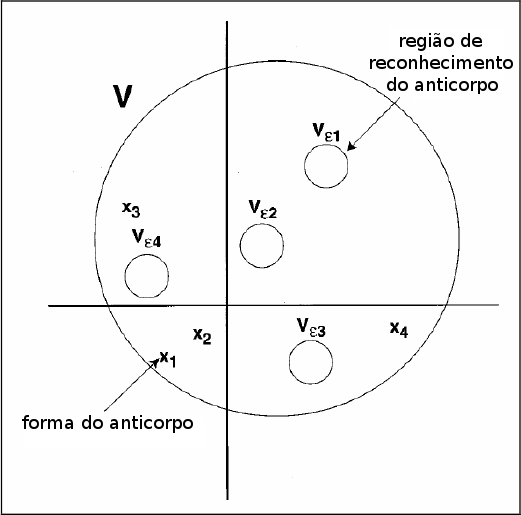
\includegraphics[width=0.75\textwidth]{img/space.png}
    \vspace{0.5cm}
    \\ Fonte: \cite{Brownlee2007}.
    \vspace{0.5cm}
\end{figure}

O espaço de formas é um hipercubo de volume V. Cada anticorpo é definido como uma área de reconhecimento nesse espaço ($\epsilon$). Na definição original, essas áreas de reconhecimento eram funções Gaussianas. A distância euclidiana entre \emph{ab} e \emph{ag} é considerada como a `afinidade' ou `medida de complementaridade'. Para isso, a natureza complementar dos anticorpos e antígenos é ignorada: uma ligação perfeita é considerada quando \emph{ab == ag}, ao contrário de \emph{ab != ag}. Anticorpos possuem uma hiper-região de reconhecimento, onde antígenos podem gerar uma resposta imune.

Uma crítica ao formalismo do espaço de formas foi feita em \citet{Carneiro1994}, destacando principalmente a simplicidade da abstração do espaço de estados e as limitações das funções de afinidade simples.

\section{Topologia de afinidade}

O objetivo de um anticorpo, no sistema imunológico, é maximizar a sua afinidade com um antígeno específico. Assim, a maturação de um anticorpo pode ser considerada também geometricamente como uma movimentação na superfície da função de afinidade para um antígeno específico \cite{Brownlee2007}.

Essa superfície teórica é geralmente considerada como contínua e possui diversos ótimos locais, ou seja, um ponto com maior afinidade que seus vizinhos, mas que não é o ponto global com maior afinidade. Esse formalismo é útil na definição e formalização do processo de maturação por hipermutação dos anticorpos, parte principal dos algoritmos baseados na teoria da seleção clonal.

Os formalismos do espaço de formas e topologia de afinidades são a base da definição do espaço de formas binário usado na seleção negativa e nas redes imunológicas, das regiões e limiares de detecção nos algoritmos de mineração de dados e classificação, e da movimentação na topologia das funções de custo nos algoritmos de otimização.

A interpretação geométrica genérica proporcionada por esses dois formalismos constitui um \emph{framework} para a investigação de princípios imunológicos, não limitada aos problemas de reconhecimento de padrões.

\section{Comparação dos algoritmos}

Garrett faz um estudo detalhado de comparação entre os principais algoritmos imunológicos \cite{Garrett2005}. Nesse trabalho, o autor define o método de comparação entre esses algoritmos em dois termos: distintividade e eficiência. A ideia por trás dessa comparação é que um algoritmo pode ser distinto de outros, mas ineficiente; como também pode ser altamente efetivo, mas redutível a outro método. No entanto, caso um método seja tanto distinto quanto efetivo, ele é realmente considerado computacionalmente útil.

Para que um algoritmo seja considerado distinto, é avaliado se seus símbolos e expressões são únicos, assim como os processos aplicados sobre estes dois, ou se podem ser transformados em símbolos, expressões ou processos de outros métodos, sem afetar a dinâmica do algoritmo. Por outro lado, para que seja considerado eficiente, é avaliado se ele obtém os resultados através de meios únicos, apresenta resultados melhores ou obtém um conjunto de resultados mais rapidamente que métodos existentes. Nessa comparação, é importante que um mesmo tipo de experimento seja executado em todos os casos, e que a mesma métrica seja aplicada na avaliação dos resultados.

\subsection{Seleção negativa}

Apesar de ser uma das mais importantes abstrações do sistema imunológico, análises de algoritmos baseados na seleção negativa demonstraram que eles sofrem de problemas de escalabilidade. Considerando o conjunto de cadeias de bits consideradas próprias (\emph{S}), o número de cadeias aleatórias (\emph{R$_{0}$}) aumenta exponencialmente com o crescimento de \emph{S}. Soma-se a isso o fato de que pode haver sobreposição nas partes do espaço de estados coberta por cada detector, enquanto outras partes podem não ser cobertas. Ou ainda podem haver áreas do espaço não-próprio que não podem ser cobertas por um detector sem que ele cubra também uma área própria.

Já foi questionada a tentativa de cobrir, aleatoriamente, um espaço não-próprio infinito utilizando detectores de tamanho finito. Como autores como Dasgupta, Forrest e Nino apontam, esse tipo de modelagem permite que múltiplos detectores identifiquem um elemento não-próprio por aproximação, além de permitir a criação de detectores sem que se tenha conhecimento do espaço de estados. De fato, caso o conjunto próprio fosse desconhecido, e existisse apenas uma função que, dado um elemento, determinasse se ele pertence ou não ao conjunto próprio, a seleção negativa seria o único método, entre os discutidos, que poderia ser aplicado.

Conforme demonstrou D’haeseleer, a seleção negativa muitas vezes não é tão efetiva quanto outras técnicas, mas oferece um nível de segurança maior por ser menos suscetível à tentativas deliberadas dos agentes maliciosos de enganar o sistema\iffalse melhorar essa frase\fi. Outras vantagens apontadas incluem a habilidade de detecção de mudanças nos eventos do sistema, de verificar mudanças em partes de um objeto sem a necessidade de verificar o objeto como um todo e de aplicar diversos detectores diferentes sobre um mesmo objeto, aumentando a probabilidade de detecção conforme o número de detectores utilizado. O autor também aponta que subconjuntos dos detectores podem ser utilizados de maneira autônoma e distribuída.

Alguns trabalhos incorporam processos da seleção clonal na seleção negativa \cite{Garrett2005}: os detectores são gerados aleatoriamente, como no algoritmo original, e aqueles que identificam elementos próprios passam pelo processo de seleção clonal. O objetivo é que esses detectores sejam ajustados até que não cubram mais o espaço próprio. A vantagem, nesse caso, é a de utilizar o poder de exploração do espaço de estados da seleção clonal para dispensar o controle determinístico complexo dos detectores feito na maior parte dos trabalhos da área.

\subsection{Seleção clonal}

A principal característica da seleção clonal, que a difere dos outros métodos, é seu mecanismo de ajuste da mutação. Enquanto nos outros métodos o grau de mutação (ou o grau em que a mutação muda) é constante, na seleção clonal esse grau é determinado por uma função baseada na aptidão da solução. Soluções com pouca derivação do estado ótimo sofrem pequenos graus de mutação. Da mesma maneira, outra característica única da seleção clonal é a função que define o número de clones de acordo com a aptidão da solução.

No entanto, algoritmos baseados na seleção clonal podem ser lentos em sua execução devido ao número de clones, que aumenta conforme a média função de aptidão aumenta. A otimização é uma área onde os algoritmos baseados na seleção clonal têm mostrado bons resultados \cite{Garrett2005}.

\subsection{Redes imunológicas artificiais}

Devido às comparações entre cada possível par de anticorpos, as redes imunológicas são, de maneira geral, lentas. Como cada anticorpo é comparado com cada um dos outros, a complexidade (em questão de tempo) é geralmente \emph{O}(\emph{n$^{2}$}). Algumas pesquisas na área tentam reduzir essa complexidade, permitindo apenas um número finito de comparações em cada iteração. No entanto, isso pode comprometer os resultados, devido ao menor número de interações entre os elementos da rede, o que parece ir contra o propósito inicial do modelo.

\subsection{Teoria do Perigo}

As dificuldades na implementação de sistemas baseados na Teoria do Perigo são as mesmas encontradas na aceitação da teoria na imunologia: a natureza dos sinais de perigo não é facilmente identificável; e o sistema aparentemente deve primeiro sofrer o dano para que as medidas de proteção possam ser tomadas.

\section{Considerações finais}

Os algoritmos apresentados nesse capítulo foram aplicados em sistemas computacionais de diversas áreas, apresentado resultados satisfatórios, em especial em sistemas de detecção. O domínio dos problemas de detecção de fraude é promissor para esses algoritmos, como a maioria dos problemas de detecção.

Os resultados dos algoritmos apresentados nas seções anteriores foram comparados com os resultados de algoritmos tradicionais da área da Inteligência Artificial. Dos algoritmos imunológicos, são usados: AIRS, Immunos e seleção clonal. Esses algoritmos foram escolhidos por serem representantes característicos da área de sistema imunológicos artificiais e por terem implementações atualizadas e disponíveis abertamente.

Para os algoritmos tradicionais, foram escolhidos aqueles que são comumente usados na área de mineração de dados. Em especial, os algoritmos genéticos, que têm características semelhantes aos imunológicos, já que ambos têm inspiração na biologia.

\begin{table}[h]
    \vspace{0.5cm}
    \centering
    \caption{Algoritmos utilizados para comparação}
    \label{tbl:ais_algs}
    \vspace{0.5cm}
    \begin{tabular}{c c}
        \hline
        Algoritmos tradicionais & Algoritmos imunológicos   \\
        \hline
        Redes neurais                & AIRS    \\
        Máquina de vetor de suporte  & Immunos \\
        Algoritmos genéticos         & CLONALG \\
        Árvores de decisão           &         \\
        Learning Vector Quantization &         \\
        \hline
    \end{tabular}
    \vspace{0.5cm}
\end{table}

Nas próximas seções, será mostrada a aplicação de três algoritmos baseados no sistema imunológico natural a conjuntos de dados de fraudes. Os resultados são então comparados com algoritmos tradicionais da inteligência artificial.

Para que essa comparação tenha utilidade prática, primeiro é necessário que se estabeleçam critérios para a avaliação do desempenho desses algoritmos. O próximo capítulo apresenta os critérios de avaliação comumente empregados na mineração de dados. Apresenta também como esses critérios devem ser adaptados para a aplicação na detecção de fraude e demonstra como estes são aplicados nesse trabalho.
